\subsection{Experiment 3: Block Effects in Cross-Validation}

\begin{figure}[H]
    \centering
    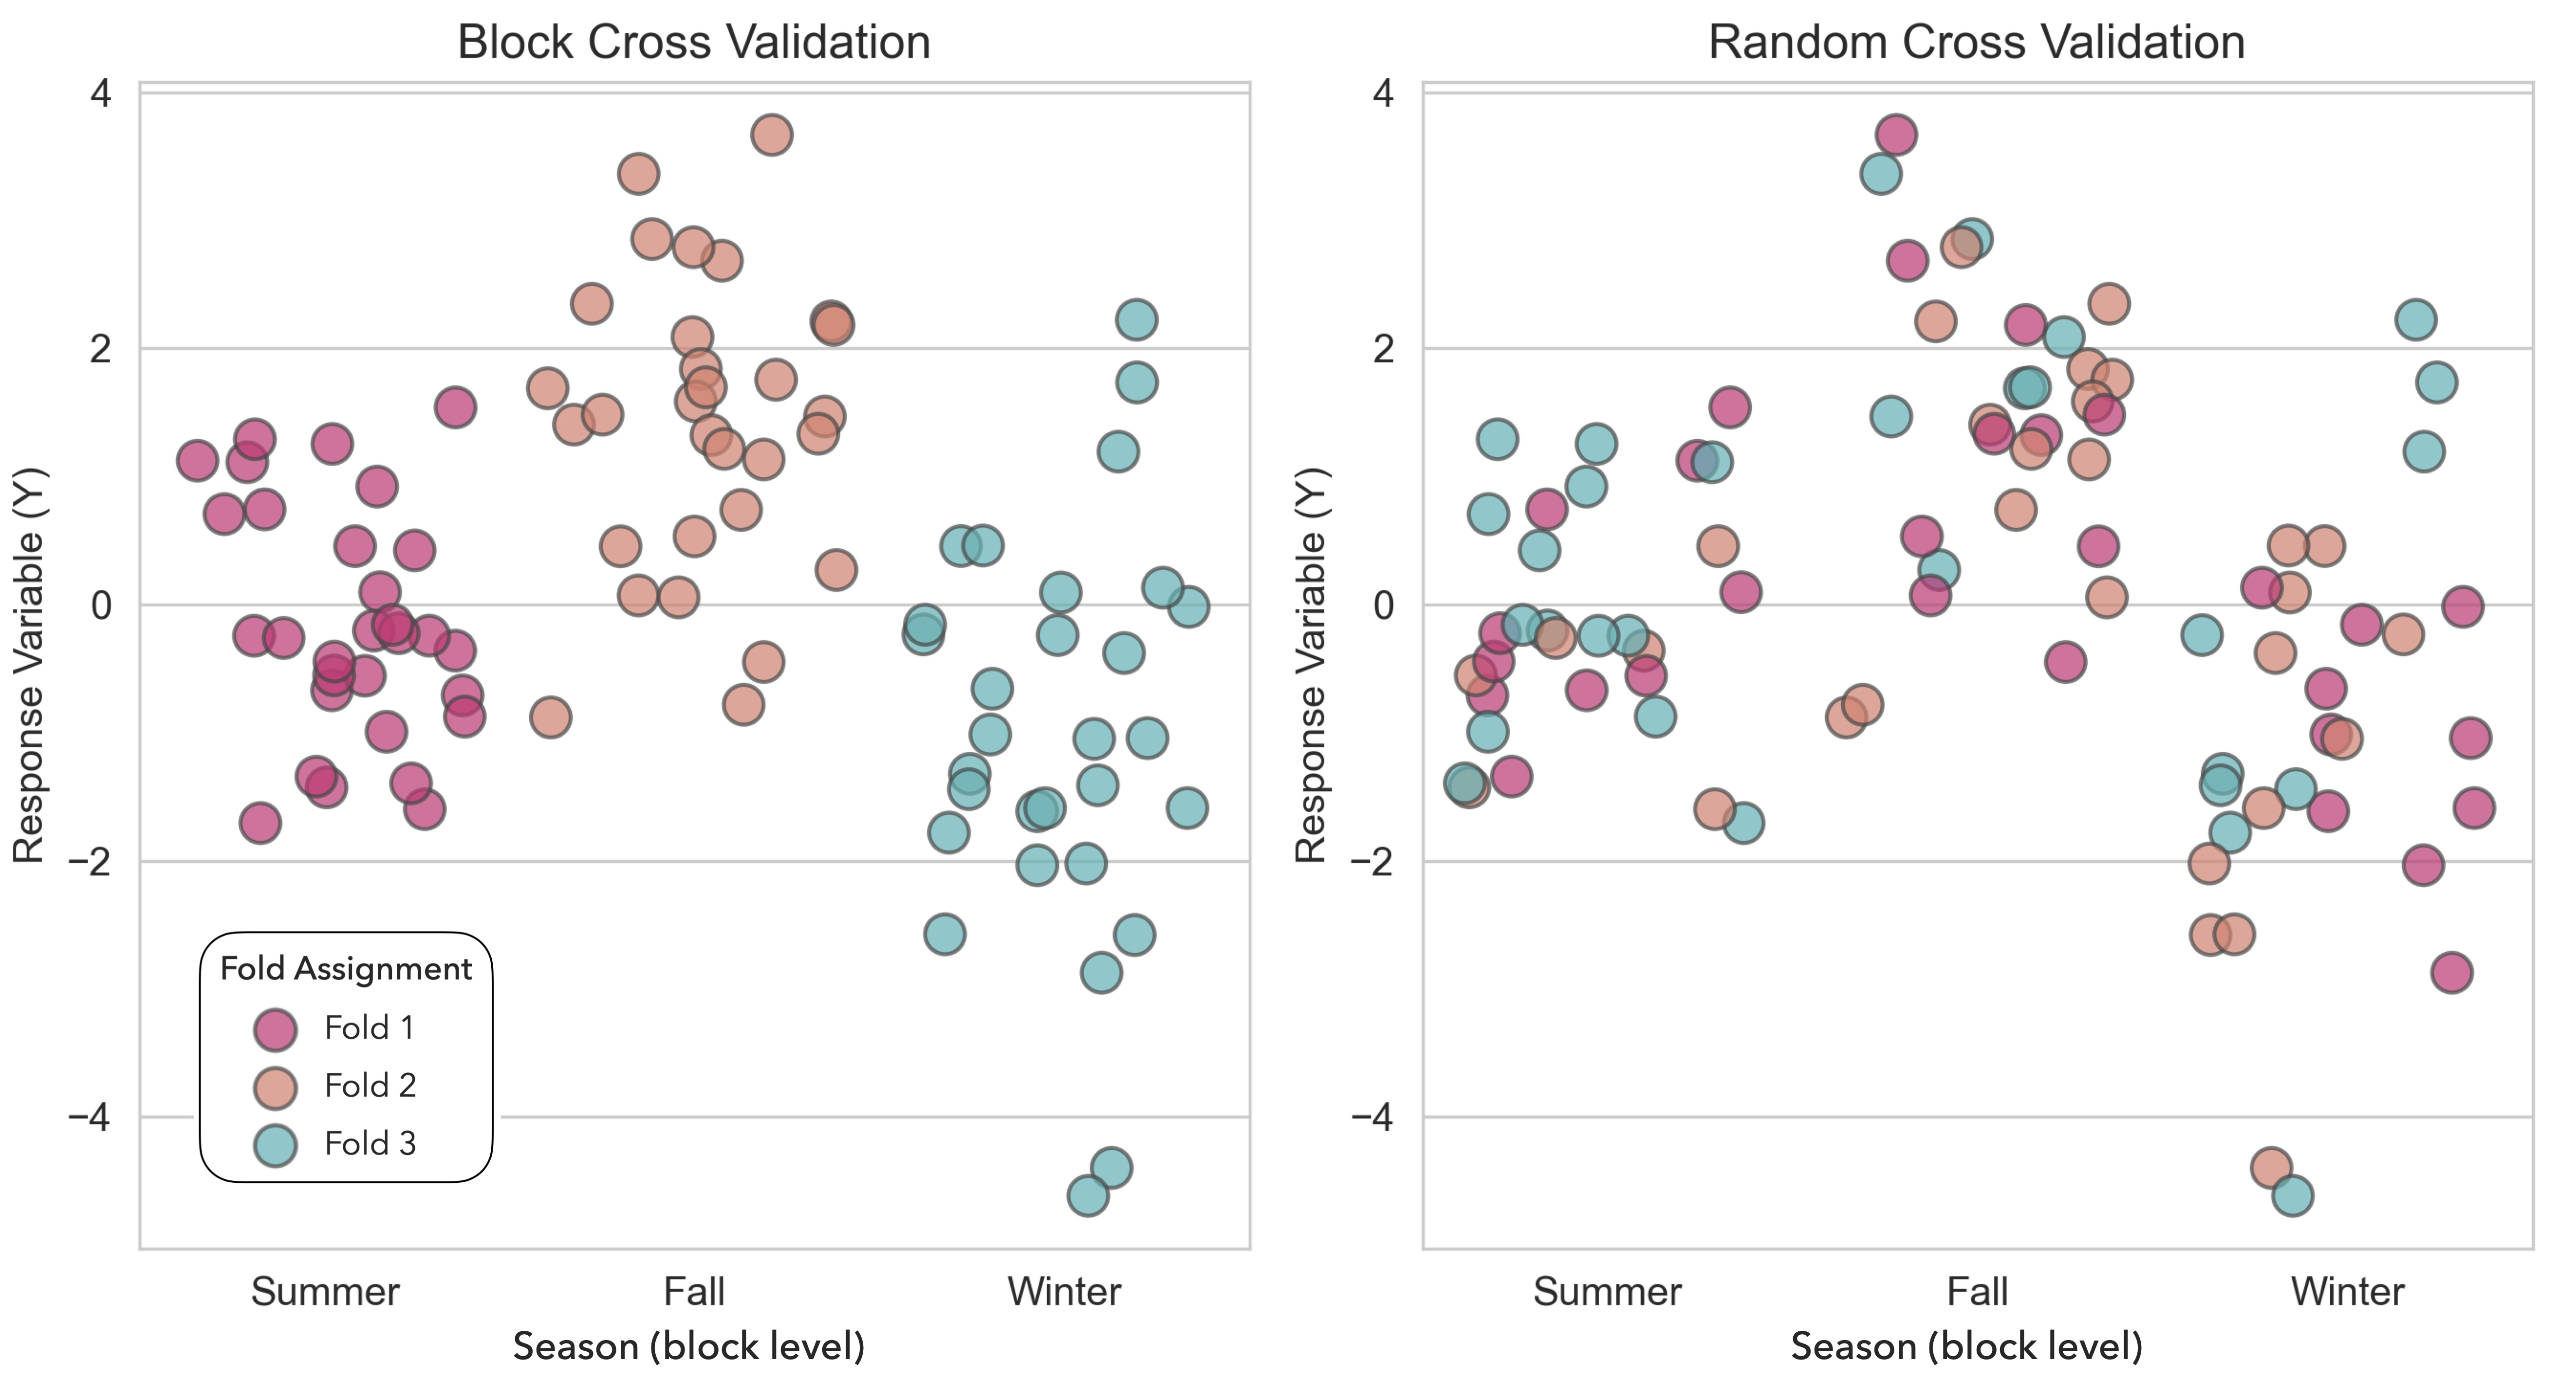
\includegraphics[width=.8\textwidth]{fig_s3_block.jpg}
    \caption{Illustration of fold assignment in block cross validation (left) and random cross validation (right). Folds are color-coded, and the block effect is set to 3 in this example.}
    \label{fig:s3_block}
\end{figure}

The objective of this experiment is to demonstrate how Random CV, which randomly assigns samples to folds without accounting for block effects, can lead to an overestimation of model performance. As a benchmark, the experiment employs Block CV, where each block is treated as a fold in cross-validation. The hypothesis is that the model performance estimated by Random CV will be significantly higher than that estimated by Block CV.

This experiment utilizes both simulated and real-world datasets, both of which were collected across multiple seasons, introducing block effects that confound both the predictor features and the response variable. The simulated dataset includes 200 observations per season, distributed equally across seasons, while the real-world dataset also contains approximately 200 observations per season. The block effect in both datasets is defined by the seasonal variation.

The experiment evaluates two model validation strategies: Block CV and Random CV, both using a 3-fold cross-validation approach. Three folds are used to match the number of seasons in the dataset. In Block CV, each block (i.e., season) is treated as a distinct fold, ensuring that samples from the same block are not split across folds. In Random CV, samples are randomly assigned to folds without consideration of block boundaries (Figure ~\ref{fig:s3_block}). The predictive model used is a random forest regression model, and its performance is assessed using Pearson’s correlation coefficient $r$ and RMSE.

The simulation is run for 500 iterations, with $X$ (predictor variables) and $Y$ (response variable) resampled in each iteration for the simulation dataset and also the fold assignment to account for variability. A one-way ANOVA was performed to evaluate whether the choice of CV strategy (i.e., block CV vs. random CV) significantly affects model bias. The model was specified as $y \sim 1 + \text{BlockCV}$,
